\documentclass{standalone}

\usepackage{tikz}

\begin{document}
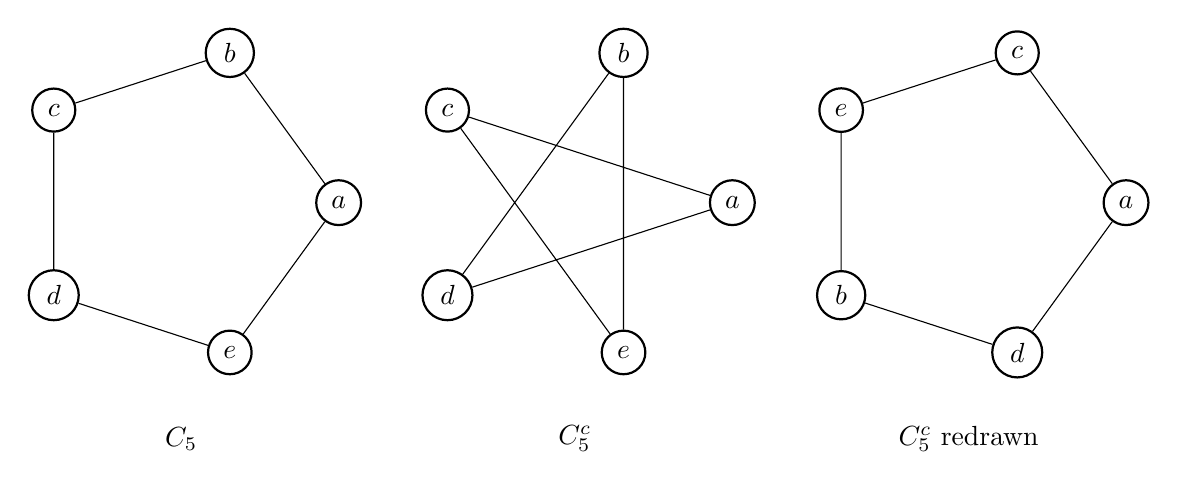
\begin{tikzpicture}
\begin{scope}[every node/.style={circle, thick, draw}]  \node (a) at (0:2cm) {$a$};
  \node (b) at (72:2cm) {$b$};
 \node (c) at (144:2cm) {$c$};
 \node (d) at (216:2cm) {$d$};
 \node (e) at (288:2cm) {$e$};
 \draw (a)--(b)--(c)--(d)--(e)--(a);
\end{scope}

\begin{scope}[xshift=5cm,every node/.style={circle, thick, draw}]  \node (a) at (0:2cm) {$a$};
 \node (b) at (72:2cm) {$b$};
 \node (c) at (144:2cm) {$c$};
 \node (d) at (216:2cm) {$d$};
 \node (e) at (288:2cm) {$e$};
 \draw (a)--(c)--(e)--(b)--(d)--(a);
\end{scope}


\begin{scope}[xshift=10cm, every node/.style={circle, thick, draw}]  \node (a) at (0:2cm) {$a$};
  \node (b) at (72:2cm) {$c$};
 \node (c) at (144:2cm) {$e$};
 \node (d) at (216:2cm) {$b$};
 \node (e) at (288:2cm) {$d$};  \draw (a)--(b)--(c)--(d)--(e)--(a);
\end{scope}

\draw (0,-3) node {$C_5$};
\draw (5, -3) node {$C_5^c$};
\draw (10cm, -3cm) node {$C_5^c$ redrawn};


\end{tikzpicture}

\end{document} 
